\documentclass[12pt]{article}
\usepackage[spanish, english, es-tabla]{babel}
\usepackage[utf8]{inputenc}
\usepackage[left = 2cm, right = 2cm, bottom = 2cm, top = 3cm]{geometry}
\usepackage{amsmath, amssymb}
\usepackage{graphicx}
\usepackage{hyperref}
\usepackage{listings}

\usepackage[dvipsnames]{xcolor}

\renewcommand{\lstlistingname}{Listado}

% https://tex.stackexchange.com/questions/60209/how-to-add-an-extra-level-of-sections-with-headings-below-subsubsection
\newcommand{\subsubsubsection}[1]{\paragraph{#1}\mbox{}\\}
\setcounter{secnumdepth}{4}
\setcounter{tocdepth}{4}

\begin{document}
	\selectlanguage{spanish}
	\title{Aplicación de técnicas de virtualización ligera para la evaluación de redes de comunicaciones \\ 
		\addvspace{10px} \large Trabajo Final de Estudios \\
		\large Ingeniería Telemática}
	\author{Enrique Fernández Sánchez \\ Universidad Politécnica de Cartagena}
	
	%% EDITAR PARA SEGUIMIENTO DE VERSIONES
	\date{Revisión 21 Mayo 2021}
	
	\maketitle
	\tableofcontents
	
	\pagebreak
	
	%%% TODO
	\section{Introduction}
	
	\pagebreak
	
	\section{\textit{Espacio de nombres} en \textit{Linux}}
	\subsection{¿Qué es un \textit{espacio de nombres}?}
	\noindent Los \textit{espacios de nombres}, o también llamados, \textit{namespaces}, son una característica del kernel de Linux que permite gestionar los recursos del kernel, pudiendo limitarlos a un proceso o grupo de procesos. Suponen una base de tecnología que aparece en las técnicas de virtualización más modernas (como puede ser Docker, Kubernetes, etc). A un nivel alto, permiten aislar procesos respecto al resto del kernel. \\
	
	\par \noindent El objetivo de cada \textit{namespaces} es adquirir una característica global del sistema como una abstracción que haga parecer a los procesos de dentro del \textit{namespace} que tienen su propia instancia aislada del recurso global.
	
	\subsection{¿Cúantos \textit{namespaces} hay?}
	\par\noindent El kernel ha estado en contaste evolución desde que 1991, cuando Linus Torvalds comenzó el proyecto, actualmente sigue muy activo y se siguen añadiendo nuevas características. El origen de los namespaces se remonta a la versión del kernel 2.4.19, lanzada en 2002. Conforme fueron pasando los años, más tipos diferentes de namespaces se fueron añadiendo a Linux. El concepto de \textit{User namespaces}, se consideró terminado con la versión 3.9.\\
	\par \noindent Actualmente, tenemos 8 tipos diferentes de namespaces, siendo el último añadido en la versión 5.8 (lanzada el 2 de Agosto de 2020). 
	
	\begin{enumerate}
		\item UTS (hostname)
		\item Mount (mnt)
		\item Process ID (pid)
		\item Network (net)
		\item User ID (user) 
		\item Interprocess Communication (ipc)
		\item Control group (cgroup)
		\item Time
	\end{enumerate}
	
	\pagebreak
	
	\subsubsection{UTS namespace}
	\par \noindent El tipo más sencillo de todos los namespaces. La funcionalidad consiste en controlar el hostname asociado del ordenador, en este caso, del proceso o procesos asignados al namespace. Existen tres diferentes rutinas que nos permiten obtener y modifcar el hostname: 
	\begin{itemize}
		\item \textit{sethostname()}
		\item \textit{setdomainname()}
		\item \textit{uname()}
	\end{itemize}
	En una situación normal sin namespaces, se modificaría una String global, sin embargo, si estamos dentro de un namespace, los procesos asociados tienen su propia variable global asignada.\\
	
	% example uts: https://medium.com/@teddyking/linux-namespaces-850489d3ccf
	% https://www.cloudsavvyit.com/742/what-are-linux-namespaces-and-what-are-they-used-for/
	\par \noindent Un ejemplo muy basico de uso de este namespaces podría ser el siguiente:\\
	\begin{lstlisting}[language=bash, caption=Example usage UTS namespace]
$ sudo su			# super user
$ hostname			# current hostname
> arch-linux					
$ unshare -u /bin/sh		# shell with UTS namespace
$ hostname new-hostname		# set hostname
$ hostname			# check hostname of the shell
> new-hostname
$ exit				# exit shell and namespace
$ hostname			# original hostname
> arch-linux
	\end{lstlisting}

	\addvspace{10px}

	\par \noindent En el ejemplo planteado, vemos que utilizamos el comando \texttt{unshare}. Utilizando la documentación de dicho comando, \texttt{man unshare}. Podemos deducir los siguiente:
	\begin{itemize}
		\item Ejecuta un programa con algunos namespaces diferentes del host.
		\item En los parametros podemos especificar cual o cuales namespaces queremos desvincular.
		\item Tenemos que especificar la ruta del ejecutable que queremos aislar
		\item La sintaxis sería tal que: \texttt{unshare [options] <program> [<argument>...]}
	\end{itemize}
	
	\pagebreak
	
	\subsubsection{Mount namespace}
	\par \noindent Un \textit{mount namespace (mnt)} supone otro tipo de espacio de nombres, en este caso relacionado con los \textit{mounts} de nuestro sistema. Lo primero es entender a que nos referimos cuando hablamos de \textit{mount}. \textit{Mount}, o montaje, hace referencia a conectar un sistema de archivos adicional que sea accesible para el sistema de archivos actual de un ordenador. Un \text{mount}, tiene asignado lo que se llama \textit{mount point}, que corresponde con el directorio en el que está accesible el sistema de archivo que previamente hemos montado.\\
	
	\par \noindent Por lo tanto, un namespace de tipo \textit{mount} nos permite modificar un sistema de archivos en concreto, sin que el host pueda ver y/o acceder a dicho sistema de archivos. Un ejemplo básico de esta funcionalidad podría ser la siguiente:
	
	\addvspace{10px}
	
	\begin{lstlisting}[language=bash, caption=Example of usage mount namespace]
$ sudo su		# run a shell in a new mount namespace
$ unshare -m /bin/sh
$ mount --bind /usr/bin/ /mnt/
$ ls /mnt/cp
> /mnt/cp
$ exit			# exit the shell and close namespace
$ ls /mnt/cp
> ls: cannot access '/mnt/cp': No such file or directory
	\end{lstlisting}

	\addvspace{10px}
	
	\par \noindent Como vemos en el ejemplo, dentro del namespaces lo que hacemos es crear un \textit{mount} de tipo \textit{bind}, que tiene por función que un archivo de la máquina host se monte en un directorio en específico, en este caso, un directorio unicamente del programa que hemos asignado al namespace. Otro ejemplo de uso de estos namespaces es crear un sistema de archivos temporal que solo sea visible para ese proceso.
	
	\pagebreak
	
	\subsubsection{Process ID namespace}
	\par \noindent Para entender en que consiste este namespace, primero tenemos que conocer la definición de \textit{process id} dentro del Kernel. En este caso, \textit{process id} hace referencia a un número entero que utiliza el Kernel para identificar los procesos de manera unívoca.\\
	
	\par \noindent Concretando, aísla el namespace de la ID del proceso asignado, dando lugar a que, por ejemplo, otros namespaces puedan tener el mismo PID. Esto nos lleva a la situación de que un proceso dentro de un \textit{PID namespace} piense que tiene asignado el ID "1", mientras que en la realidad (en la máquina host) tiene otro ID asignado.
	
	\addvspace{10px}
	
	\begin{lstlisting}[language=bash, caption=Example of usage process id namespace]
$ echo $$		# PID de la shell
$ ls -l /proc/$$/ns	# ID espacios de nombres 
$ sudo unshare -f --mount-proc -p /bin/sh
$ echo $$		# PID de la shell dentro del ns
$ ls -l /proc/$$/ns	# nuevos ID espacio de nombres
$ ps

$ ps -ef 		# ejecutar en una shell fuera del ns. Comparar PID
$ exit
	\end{lstlisting}

	\addvspace{10px}
	
	\par \noindent Si ejecutamos el ejemplo, lo que podemos comprobar es que el ID del proceso que está dentro del namespaces (\texttt{echo \$\$}), no coincide con el proceso que podemos ver de la máquina host (\texttt{ps -ef | grep /bin/sh}). Más concretamente, el primer proceso creado en un PID namespace recibirá el pid número 1, y además de un tratamiento especial ya que supone  un \texttt{init process} dentro de ese namespace.
	
	% revisar: https://www.redhat.com/sysadmin/linux-pid-namespaces
	% https://man7.org/linux/man-pages/man7/pid_namespaces.7.html
	
	\pagebreak
	
	\subsubsection{Network namespace}
	\par \noindent Este namespaces nos permite aislar la parte red de una aplicación o proceso que nosotros elijamos. Con esto conseguimos que el \textit{stack} de red de la máquina host sea diferente al que tenemos en nuestro namespace. Debido a esto, el namespace crea una interfaz virtual, conjunto con el resto de necesidades para conformar un stack de red completo (tabla de enrutamiento, tabla ARP, etc...).\\
	
	\par \noindent Para crear un \textit{namespace} de tipo \textit{network}, y que este sea persistente, utilizamos la \textit{tool} ip (del \textit{package} iproute2).
	\begin{lstlisting}[language=bash, caption=Creation persistent network namespace]
$ ip netns add ns1
	\end{lstlisting}

	\par \noindent Este comando creará un network namespace llamado ns1. Cuando se crea dicho namespace, el comando ip realiza un montaje tipo bind en la ruta /var/run/netns, permitiendo que el namespace sea persistente aún sin tener un proceso asociado.
	\begin{lstlisting}[language=bash, caption=Comprobar network namespaces existentes]
$ ls /var/run/netns
or
$ ip netns
	\end{lstlisting}
	
	\addvspace{10px}

	\par \noindent Como ejemplo, podemos proceder a añadir una interfaz de \textit{loopback} al namespace que previamente hemos creado:
	\begin{lstlisting}[language=bash, caption=Asignar interfaz loopback a un namespace]
$ ip netns exec ns1 ip link dev lo up
$ ip netns exec ns1 ping 127.0.0.1
> PING 127.0.0.1 (127.0.0.1) 56(84) bytes of data. 
> 64 bytes from 127.0.0.1: icmp_seq=1 ttl=64 time=0.115 ms
	\end{lstlisting}

	\par \noindent La primera línea de este ejemplo, corresponde con la directiva que le dice al namespace que "levante" la interfaz de loopback. La segunda línea, vemos como el namespace ns1 ejecuta el ping a la interfaz de loopback (el loopback de ese namespace).
	
	\addvspace{10px}
	
	\par \noindent Es importante mencionar, que aunque existen más comandos para gestionar las redes dentro de linux (como pueden ser ifconfig, route, etc), el comando ip es el considerado sucesor de todos estos, y los anteriores mencionados, dejarán de formar parte de Linux en versiones posteriores. Un detalle a tener en cuenta con el comando ip, es que es necesario tener privilegios de administrador para poder usarlo, por lo que deberemos ser root o utilizar sudo.
	
	\addvspace{10px}
	
	\par \noindent Por lo tanto, utilizando el comando ip, podemos recapitular que si utilizamos la siguiente directiva, podemos ejecutar el comando que nosotros indiquemos, pero dentro del network namespace que previamente hemos creado.
	\begin{lstlisting}[language=bash, caption=Ejecutar cualquier programa con un network namespace]
$ ip netns exec <network-namespace> <command>
	\end{lstlisting}

	\pagebreak
	
	\subsubsubsection{Ejemplo práctico}
	\par \noindent Una de las problemáticas que supone el uso de los network namespaces, es que solo podemos asignar \textbf{una interfaz} a \textbf{un namespace}. Suponiendo el caso en el que el usuario root tenga asignada la interfaz eth0 (identificador de una interfaz de red física), significaría que solo los programas en el namespace de root podrán acceder a dicha interfaz. En el caso de que eth0 sea la salida a Internet de nuestro sistema, pues eso conllevaría que no podríamos tener conexión a Internet en nuestros namespaces. La solución para esto reside en los \textbf{veth-pair}.
	
	\addvspace{10px}
	
	\par \noindent Un veth-pair funciona como si fuera un cable físico, es decir, interconecta dos dispositivos, en este caso, interfaces virtuales. Consiste en dos interfaces virtuales, una de ellas asignada al root namespace, y la otra asignada a otro network namespace diferente. Si a esta arquitectura le añadimos una configuración de IP válida y activamos la opción de hacer NAT en el eth0 del host, podemos dar conectividad de Internet al network namespace que hayamos conectado.
	
	\addvspace{10px}
	
	\begin{lstlisting}[language=bash, caption=Ejemplo configuración de NAT entre eth0 y veth]
# Remove namespace if exists
$ ip netns del ns1 &>/dev/null

# Create namespace
$ ip netns add ns1

# Create veth link
$ ip link add v-eth1 type veth peer name v-peer1

# Add peer-1 to namespace.
$ ip link set v-peer1 netns ns1

# Setup IP address of v-eth1
$ ip addr add 10.200.1.1/24 dev v-eth1
$ ip link set v-eth1 up

# Setup IP address of v-peer1
$ ip netns exec ns1 ip addr add 10.200.1.2/24 dev v-peer1
$ ip netns exec ns1 ip link set v-peer1 up
# Enabling loopback inside ns1
$ ip netns exec ns1 ip link set lo up

# All traffic leaving ns1 go through v-eth1
$ ip netns exec ns1 ip route add default via 10.200.1.1
	\end{lstlisting}

	\addvspace{10px}

	\par \noindent Siguiendo el ejemplo propuesto, llegamos hasta el punto en el que el tráfico saliente del namespace ns1, será redirigido a v-eth1. Sin embargo, esto no es suficiente para tener conexión a Internet. Tenemos que configurar el NAT en el eth0.
	
	\pagebreak
	
	\begin{lstlisting}[language=bash, caption=Configuración de NAT para dar Internet a un network namespace]
# Share internet access between host and NS

# Enable IP-forwarding
$ echo 1 > /proc/sys/net/ipv4/ip_forward

# Flush forward rules, policy DROP by default
$ iptables -P FORWARD DROP
$ iptables -F FORWARD

# Flush nat rules.
$ iptables -t nat -F

# Enable masquerading of 10.200.1.0 (ip of namespaces)
$ iptables -t nat -A POSTROUTING -s 10.200.1.0/255.255.255.0 -o eth0 
	-j MASQUERADE

# Allow forwarding between eth0 and v-eth1
$ iptables -A FORWARD -i eth0 -o v-eth1 -j ACCEPT
$ iptables -A FORWARD -o eth0 -i v-eth1 -j ACCEPT
	\end{lstlisting}
	
	\addvspace{10px}
	
	\par \noindent Si todo lo hemos configurado correctamente, ahora podríamos realizar un ping hacia Internet, y este nos debería resultar satisfactorio.
	\begin{verbatim}
$ ip netns exec ns1 ping google.es
> PING 8.8.8.8 (8.8.8.8) 56(84) bytes of data.
> 64 bytes from 8.8.8.8: icmp_seq=1 ttl=50 time=48.5ms
> 64 bytes from 8.8.8.8: icmp_seq=2 ttl=50 time=58.5ms
	\end{verbatim}

	\addvspace{10px}
	
	\par \noindent Aún así, no resulta muy comodo el utilizar \colorbox{Lavender}{\textit{ip netns exec}} seguido de la aplicación a utilizar. Es por esto por lo que es común ejecutar dicho comando para asignar el network namespace a una shell. Esto sería tal que así:
	\begin{verbatim}
$ ip netns exec ns1 /bin/bash
	\end{verbatim}
	\par \noindent Utilizaremos \colorbox{Lavender}{\textit{exit}} para salir de la shell y abandonar el network namespace.


	% https://blogs.igalia.com/dpino/2016/04/10/network-namespaces/
	
	\pagebreak
	\subsubsection{User ID (user)}
	\par \noindent Cada sistema dispone de una manera de monitorizar que usuario es el dueño de cada archivo. Esto permite al sistema restringir el acceso a aquellos archivos que consideramos sensibles. Además, bloquea el acceso entre diferentes usuarios dentro del mismo sistema. Para el usuario, este identificador de usuarios se muestra como el usuario que en ese momento está conectado, sin embargo, para nuestro sistema, el identificador de usuario esta compuesto por una combinación arbitraria de caracteres alfanuméricos. Con el fin de mantener el monitoreo correctamente, hay un proceso encargado de transformar esos caracteres a un número específico de identificación (UID), como por ejemplo sería 1000. Es este valor el que se asocia con los archivos creados por este usuario. Esto nos aporta la ventaja de que, si un usuario cambia su nombre, no es necesario reconstruir el sistema de archivos, ya que su UID sigue siendo 1000.\\
	
	\par \noindent Si por ejemplo queremos ver el UID del usuario que estamos usando en este momento, podemos ejecutar: \textit{echo \$UID}, el cual nos devolverá el número asociado a nuestro usuario, en mi caso es el 1000.\\
	
	\par \noindent Además de diferenciar entre los IDs de usuarios (UID), también se nos permite separar entre IDs de grupos (GID). En linux, un grupo sirve para agrupar usuarios de modo que un grupo puede tener asociado un privilegio que le permite usar un recurso o programas.\\
	
	\par \noindent Por lo tanto, el namespace de UID, lo que nos permite es tener un UID y GID diferente al del host. 
	
	\begin{lstlisting}[language=bash, caption=Ejemplo de uso UID namespace]
$ ls -l /proc/$$/ns		# espacios de nombres originales
$ id
> uid=1000(user) gid=1000(user) groups=1000(user), ...
$ unshare -r -u bash	# Crea un namespace de tipo usuario, programa bash
$ id
> uid=0(root) gid=0(root) groups=0(root),65534(nobody)
$ cat /proc/$$/uid_map
>          0       1000          1
$ cat /etc/shadow		# No nos deja acceder
> cat: /etc/shadow: Permission denied
$ exit
	\end{lstlisting}
	
	\addvspace{20px}
	
	\par \noindent Como vemos en el ejemplo, el UID de usuario difiere de la máquina host. Dentro del namespace, tenemos UID 0, sin embargo, eso no significa que podamos acceder a los archivos con UID 0 de la máquina host, ya que en verdad lo que hace el namespace es \textit{mapear} el UID 1000 al 0.
	
	\pagebreak
	
	\subsubsection{Interprocess Communication namespace (IPC)}
	\par \noindent Este namespace supone uno de los más técnicos, complicados de entender y explicar. IPC (Interprocess comunication) controla la comunicación entre procesos, utilizando zonas de la memoría que están compartidas, colas de mensajes, y semáforos. La aplicación más común para este tipo de gestión es el uso en bases de datos.
	
	\subsubsection{Control group (cgroup)}
	\par \noindent Los grupos de control, cgroups, de Linux suponen un mecanismo para controlar los diferentes recursos de nuestro sistema. Cuando CGroups están activos, pueden controlar la cantidad de CPU, RAM, acceso I/O, o cualquier faceta que un proceso puede consumir. Además, permiten definir jerarquías en las que se agrupan, de manera en la que el administrador del sistema puede definir como se asignan los recursos o llevar la contabilidad de los mismos.\\
	
	\par \noindent Por defecto, los CGroups se crean en el sistema de archivos virtual /sys/fs/cgroup. Si creamos un namespace de tipo CGroups, lo que estamos haciendo es mover el espacio de archivos virtual de dicho CGroup. Un ejemplo de esto sería, creamos un CGroup namespace en el root /sys/fs/cgroup/mycgroup. El host verá lo siguiente /sys/fs/cgroup/mycgroup/\{group1, group2, group3\}, sin embargo, el namespace solo verá \{group1, group2, group3\}. Esto es así ya que aporta seguridad a un namespace ya que los procesos del namespace solo pueden acceder a su sistema de archivos.
	
	\addvspace{60px}
	
	\begin{figure}[h]
		\begin{center}
			% https://8gwifi.org/docs/linux-namespace.jsp
			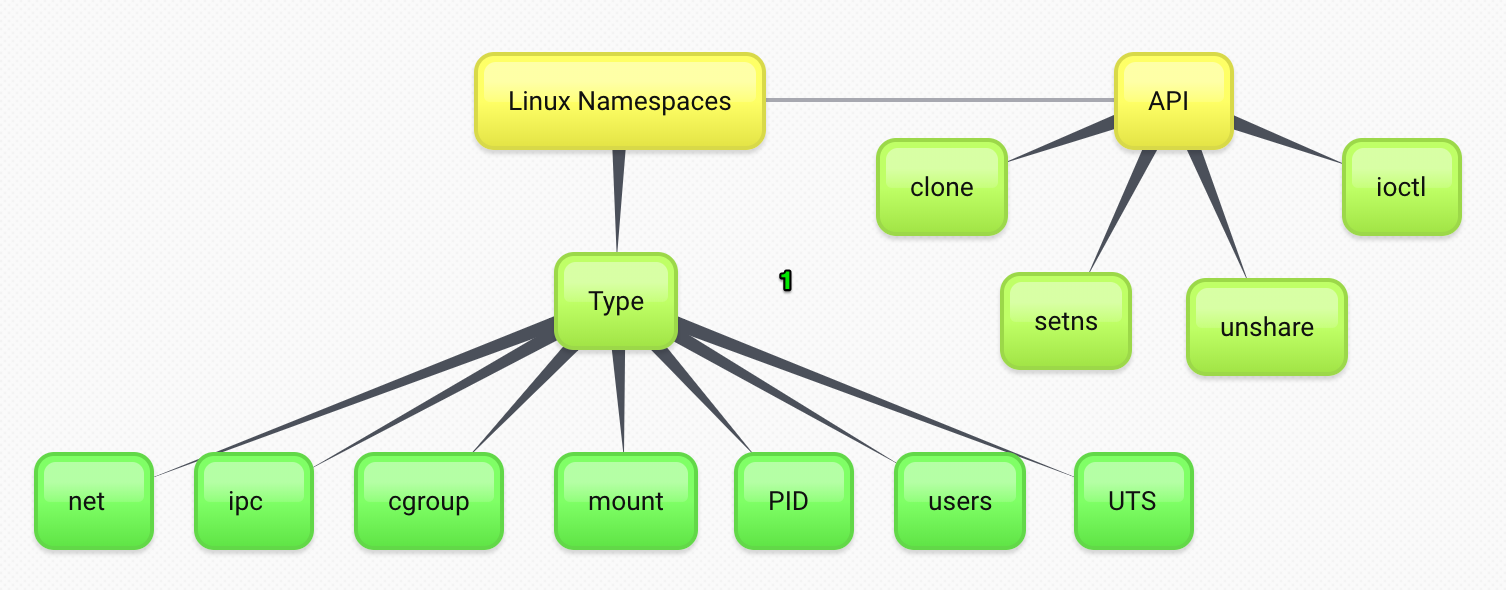
\includegraphics[width=1\textwidth]{img/linux-namespace1.png}
			\caption{Diferentes namespaces en Linux y su API de acceso.}
		\end{center}
	\end{figure}
	
	
	\pagebreak
	\subsubsection{Time}
	\par \noindent
	
	\pagebreak
	
	% Imagen namespaces: https://twitter.com/b0rk/status/1240364585766576128/photo/1
	
	\pagebreak
	
	\section{Containers LXC}
	\section{Docker}
	\section{Evaluación de prestaciones}
	\section{Interconexión física de diferentes red virtuales}
	\section{Openflow OKO}
	
	%%% Glosario
	\pagebreak
	\section{Glosario de términos}
	\begin{itemize}
		\item Namespace. \textit{Espacio de nombres}
		\item Linux. \textit{Sistema operativo tipo UNIX, de codigo abierto, multiplataforma, multiusuario y multitarea.}
		\item Kernel de linux. \textit{Núcleo del sistema operativo Linux.}
		\item PID. \textit{Process Identifier}
		\item root. \textit{Cuenta superusuario del sistema operativo Linux.}
		\item veth-pair. \textit{Virtual Ethernet Pair}
		\item UID. \textit{Identificador de usuario.}
		\item GID. \textit{Identificador de grupo.}
	\end{itemize}

	%%% Bibliography
	\pagebreak
	\section{Bibliografía}
	\subsection{Enlaces y referencias}
	%%\hyperref[bib:link1]{\emph{Reference of bibliography}}
	\begin{enumerate}
		%1
		\item 
		\label{bib:link1} \href{https://lwn.net/Articles/531114/}{\textit{Namespaces}}
		
		%2
		\item 
		\label{bib:link2} \href{https://laurel.datsi.fi.upm.es/~ssoo/SOA/namespaces.html}{Tutorial: Espacio de nombres en Linux}
		
		%3
		\item 
		\label{bib:link3} \href{https://www.phoronix.com/scan.php?page=news_item&px=Linux-Time-Namespace-Coming}{\textit{Time namespaces coming to linux}}
		
		%4
		\item 
		\label{bib:link4} \href{https://platform.sh/blog/2020/the-container-is-a-lie/}{\textit{Container is a lie. Namespaces}}
		
		%5
		\item 
		\label{bib:link5} \href{https://locurastecnicas.blogspot.com/2020/09/linux-namespaces-y-cgroups.html}{\textit{Namespaces.} Uso de \textit{cgroups}.}
		
		%6
		\item 
		\label{bib:link6} \href{https://www.youtube.com/watch?v=_WgUwUf1d34}{\textit{Introduction to Network Namespaces}}
		
		
		%7
		\item
		\label{bib:link7} \href{https://www.redhat.com/sysadmin/mount-namespaces}{\textit{Build a container by hand: the mount namespace}}
		
		
		%8
		\item
		\label{bib:link8}
		\href{https://en.wikipedia.org/wiki/Process_identifier}{Indentificador de procesos (\textit{process id})}
		
		
		%9
		\item
		\label{bib:link9}
		\href{https://www.redhat.com/sysadmin/linux-pid-namespaces}{\textit{Linux PID namespaces work with containers}}
		
		%10
		\item
		\label{bib:link10}
		\href{https://blogs.igalia.com/dpino/2016/04/10/network-namespaces/}{\textit{Network Namespaces}}
		
		%11
		\item
		\label{bib:link11}
		\href{https://developers.redhat.com/blog/2018/10/22/introduction-to-linux-interfaces-for-virtual-networking#veth}{\textit{Introduction to Linux interfaces for virtual networking. VETH}}
		
		
		%11
		\item
		\label{bib:link12}
		\href{https://elpuig.xeill.net/Members/vcarceler/articulos/introduccion-a-los-grupos-de-control-cgroups-de-linux}{\textit{Introducción a los grupos de control (cgroups) de Linux}}
		
		
		% X
		\item
		\label{bib:link20}
		\href{https://jsitech1.gitbooks.io/meet-docker/content/fundamentos_de_docker.html}{Fundamentos de Docker}
		
	\end{enumerate}
\end{document}